\autsubsection{ESA's Deep Space Communication Network}{Gustavo Feijóo Carrillo}

The International Telecommunications Union (ITU) defines Deep Space (DS) to start at a distance of 2 million km from the Earth's surface. Allocated frequency bands for DS operation according to ITU are:

\begin{itemize}
    \item S-Band: 2110-2120 MHz uplink, 2290-2300MHz downlink.
    \item X-Band: 7145-7190 MHz uplink, 8400-8450MHz downlink.
    \item Ka-Band: 34.2-34.7 GHz uplink, 31.8-32.3GHz downlink.
\end{itemize}

\noindent
ESA's effor to carry out interplanetary missions like Rosetta or Kepler Observatory as well as Icy Moon Exploration (JUICE). The capability of supporting present and future DS missions is the consequence of well established plan to expand the network of $15m$ tracking antennas into the deep space distances. The plan consisting on deploying three $35m$ DS antennas over the world, ensuring around the clock coverage to all interplanetary missions, which has been recently completed. These three DS antennas, DSA1 located in New Norcia (Australia), DSA2 in Cebreros (Spain) and DSA3 in Malargue (Argentina), are in operation since 2002, 2005 and 2013 respectively.

The DSA1-3 network will provide telecommand and telemetry links for a Europa mission but as important as the data links, is the tracking of the SC since the DSA-2 is equipped with Delta DOR (Delta Differential One-Way Ranging) capability, a new technology enabling highly precise spacecraft location and tracking.

\begin{figure}[htb]
	\centering
	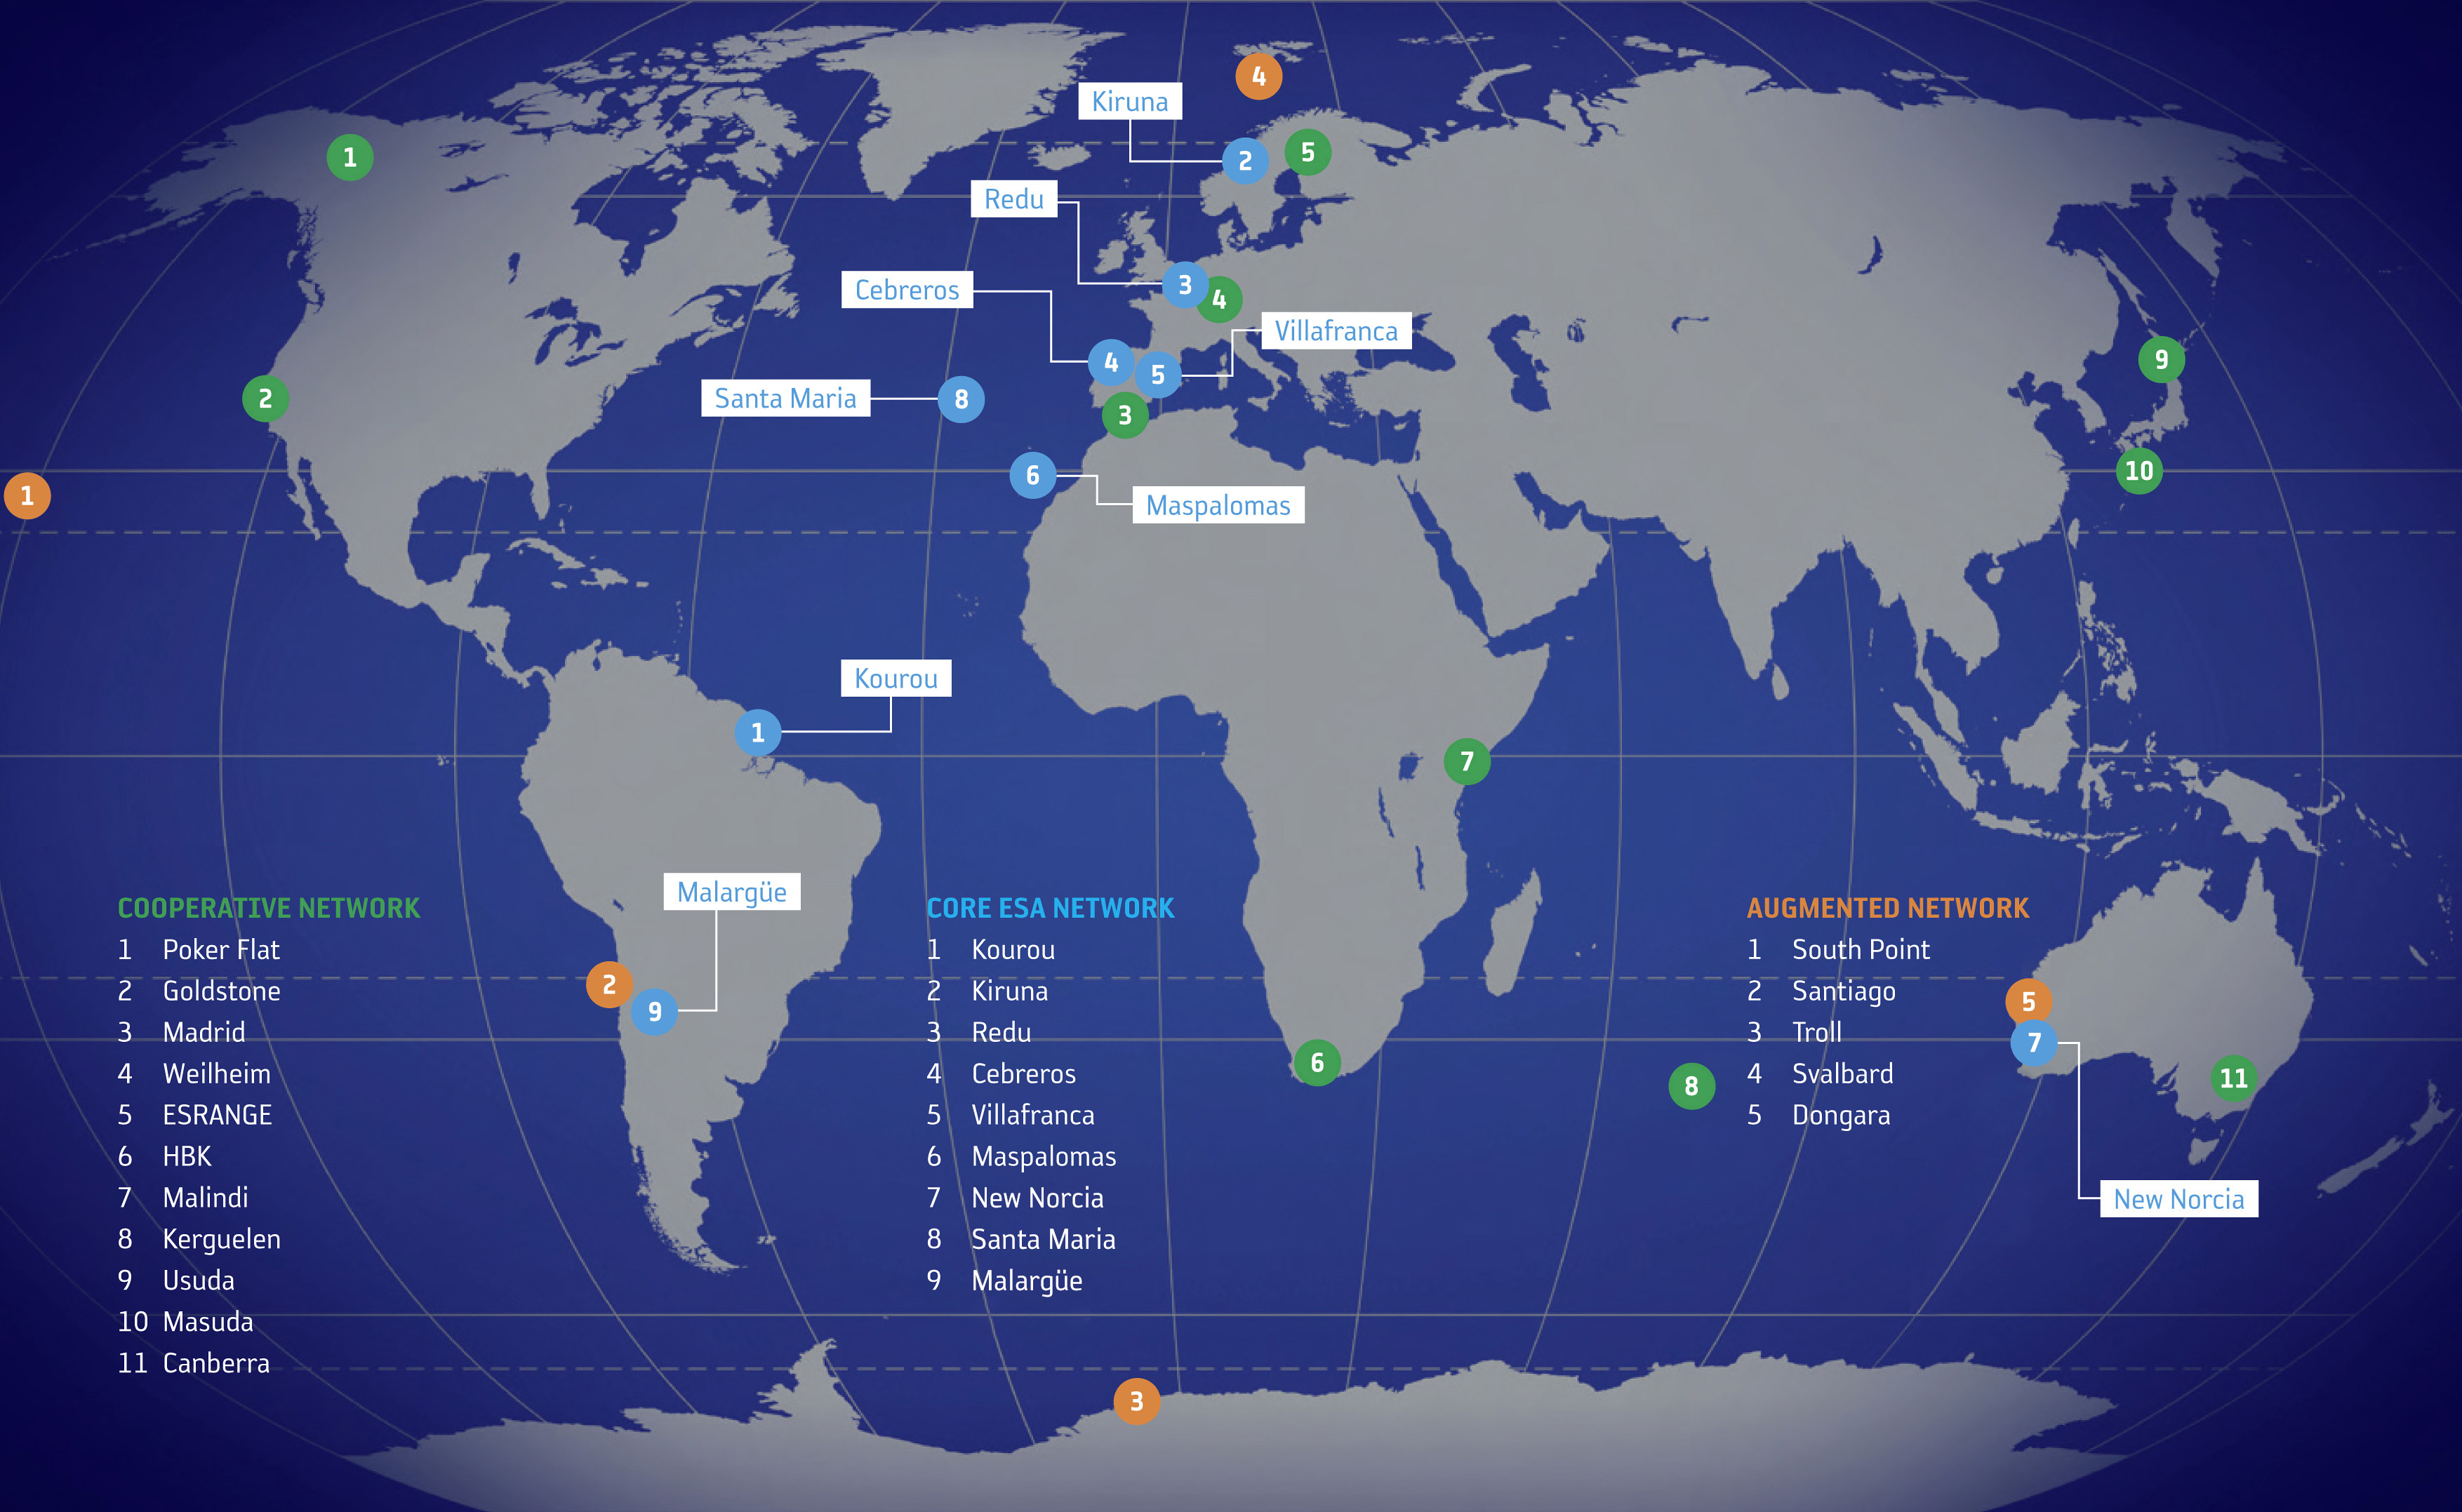
\includegraphics[width=\textwidth]{figures/comms/ESTRACK-map}
	\caption{Map of ESA's ESTRACK network, allowing for deep space communication and tracking of the spacecraft.}
	\label{fig:ESTRACK-map}
\end{figure}

\paragraph{Description}
The telecommunication system will use redundant X and Ka transponders for telemetry reception and transmission. The amplifiers will be based on redundant $65W_{RF}$, travelling wave tube amplifiers for Ka-band, and $75W_{RF}$ for X-band, respectively. The downlink of the science telemetry would be in either X-band, or Ka-band, or with both systems operating simultaneously, in the case of making up for lost transmission windows in order to meet the baseline data volume. The high gain antenna will be fixed with a diameter of $3.2m$. A medium gain antenna would be based on a horn antenna with an opening angle of the $20^o$,which covers the maximum angular distance of the Earth from the Sun, when seen from Jupiter, and would therefore allow the MGA to be simply Sun-pointed during safe mode.

A two-axis steerable medium gain antenna (MGA) is to be provided to allow for communications during the path of the inner Solar System to perform gravity assist maneuvers around Venus requiring the HGA to be used as a thermal shield for Sun as well as Venus albedo. Furthermore, for distances $>2AU$ during the interplanetary phase, and during the Jupiter phase, the MGA would be used for Earth search during safe mode recovery.

\begin{figure}[htb]
	\centering
	\subfloat[DSA-2 at Cebreros-Spain]{
		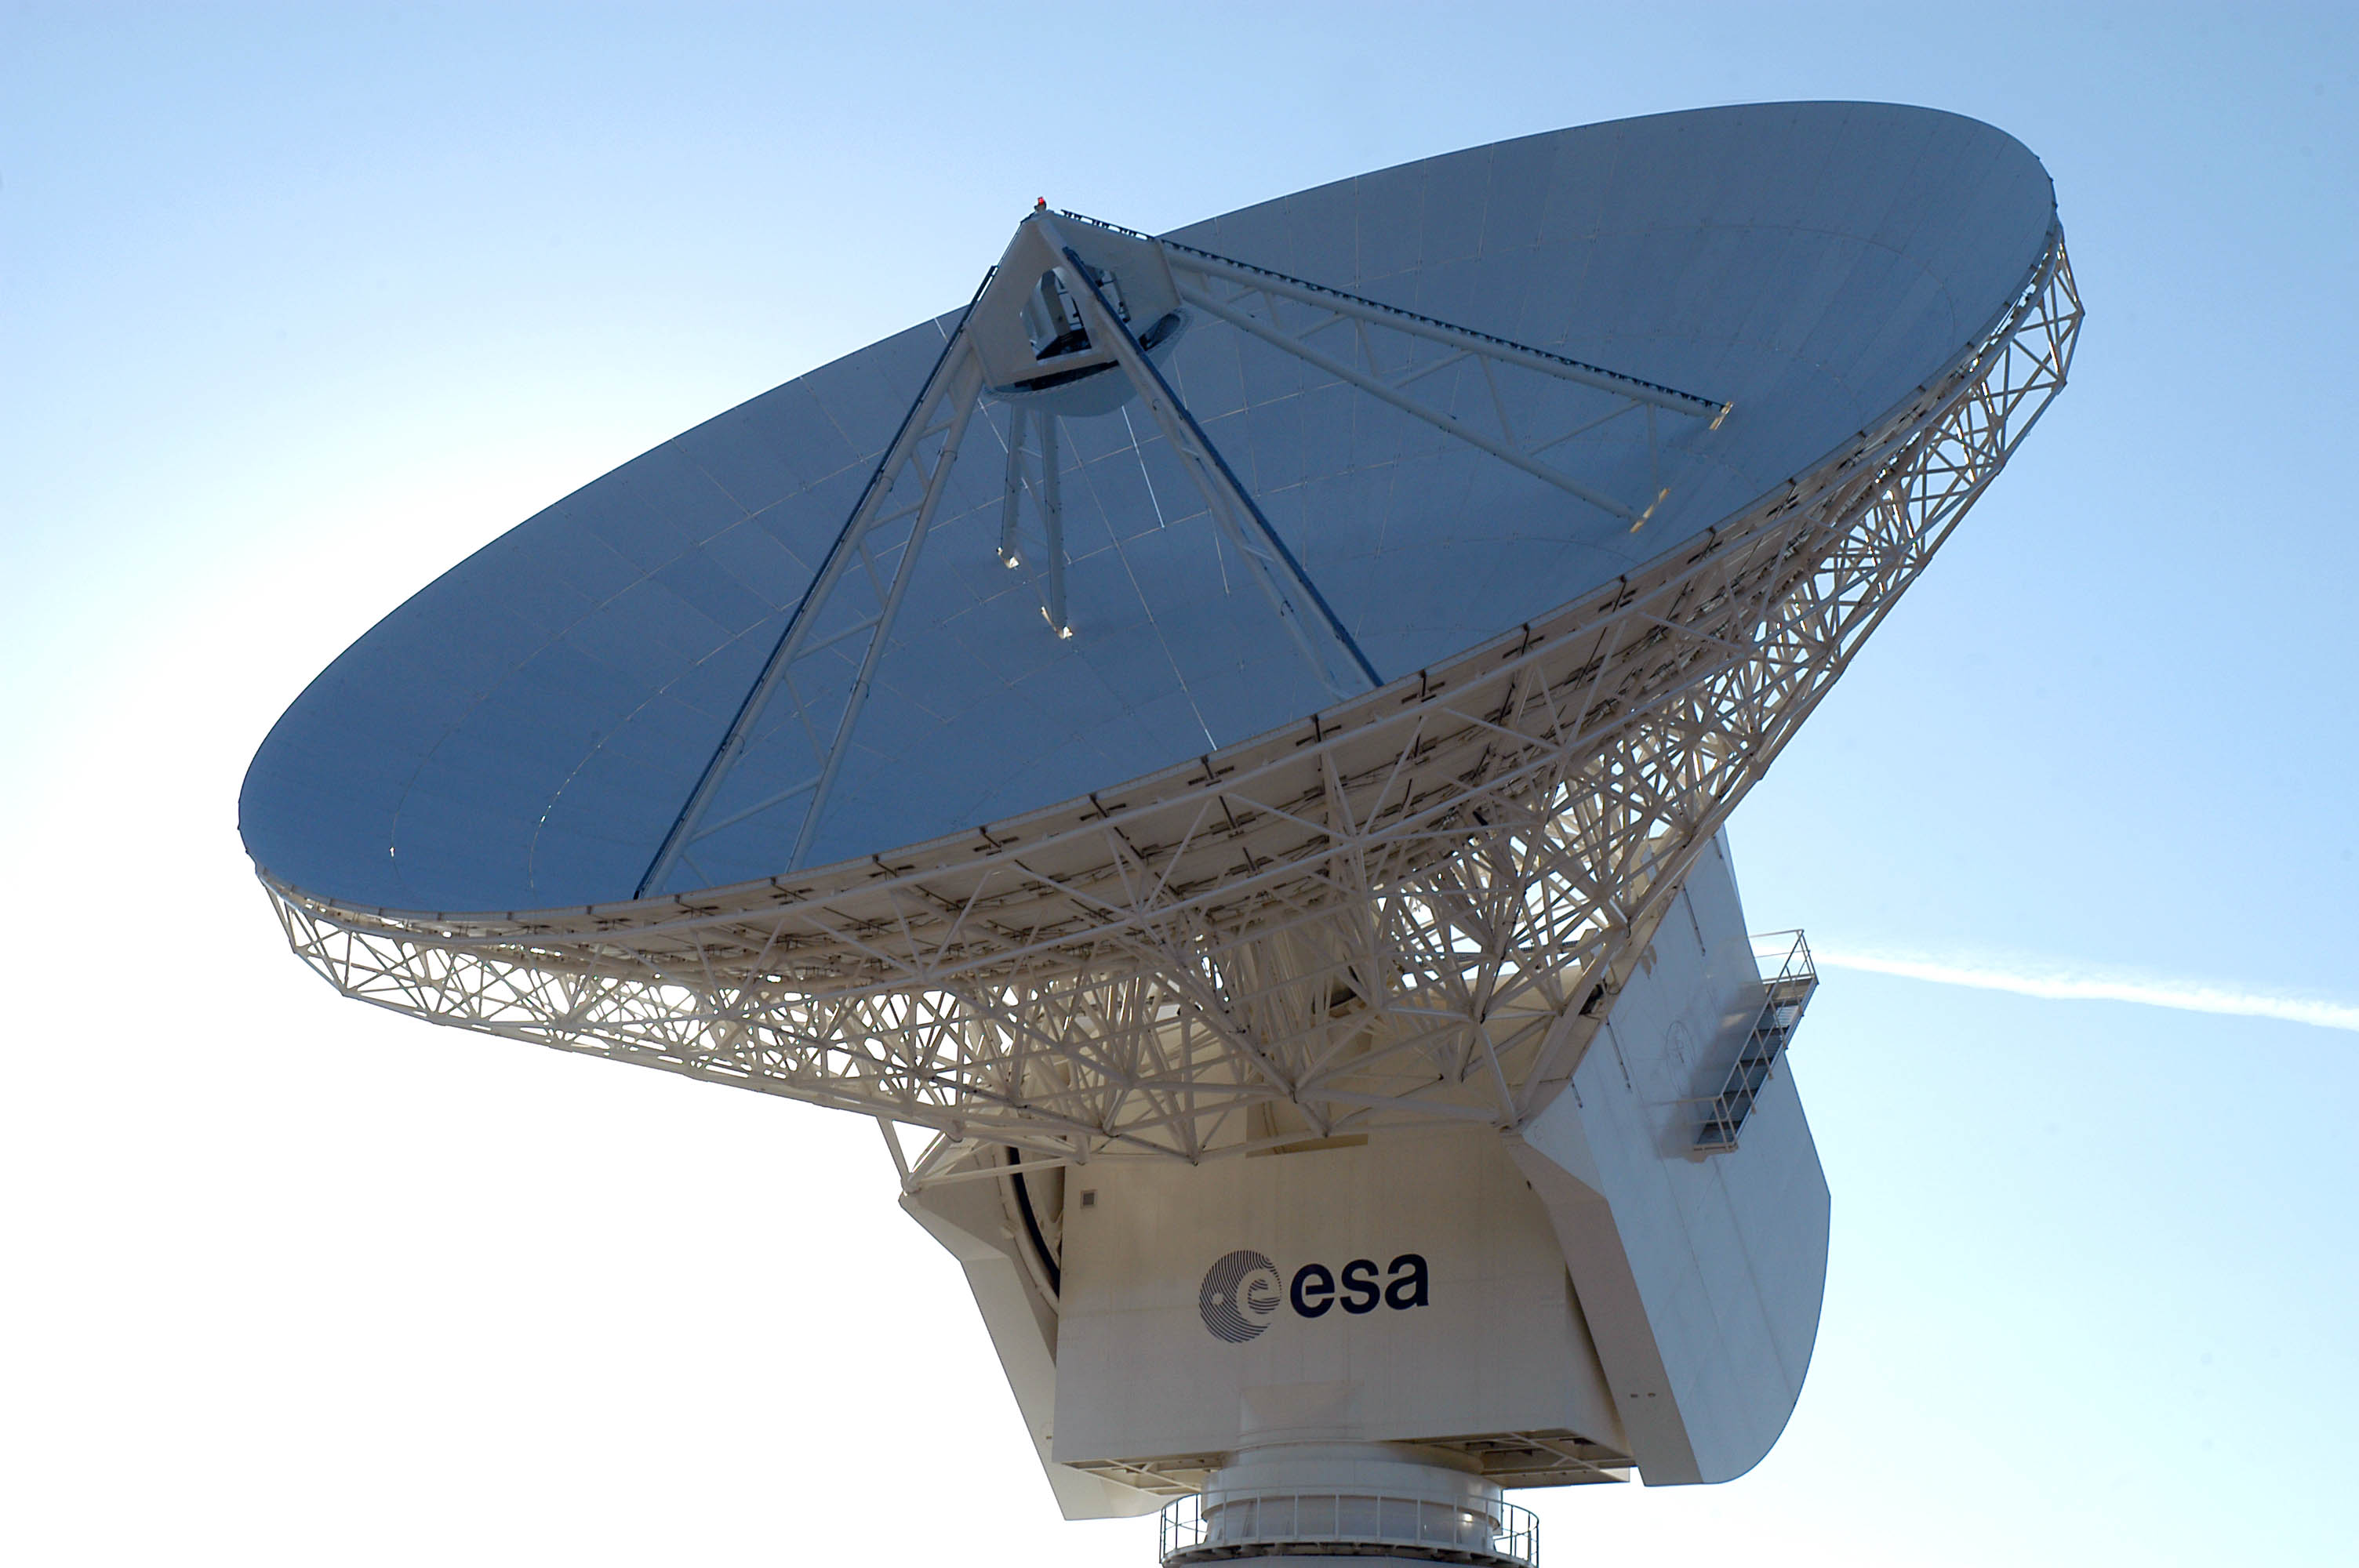
\includegraphics[width=.48\textwidth]{figures/comms/DSA2}
		\label{fig:DSA2}
	}
	\subfloat[HGA on an orbiter SC]{
		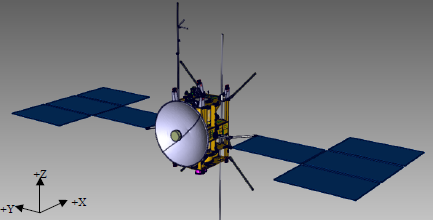
\includegraphics[width=.48\textwidth]{figures/comms/orbiter-HGA}
		\label{fig:orbiter-HGA}
	}
	\caption{Picture of $35m$ DSA and depiction of fixed HGA for DS communication and tracking of the spacecraft.}
	\label{fig:DS-a}
\end{figure}

\subsubsection{X- and Ka-band Link Budget}

\begin{figure}[htb]
	\centering
	\subfloat[X-band link budget]{
		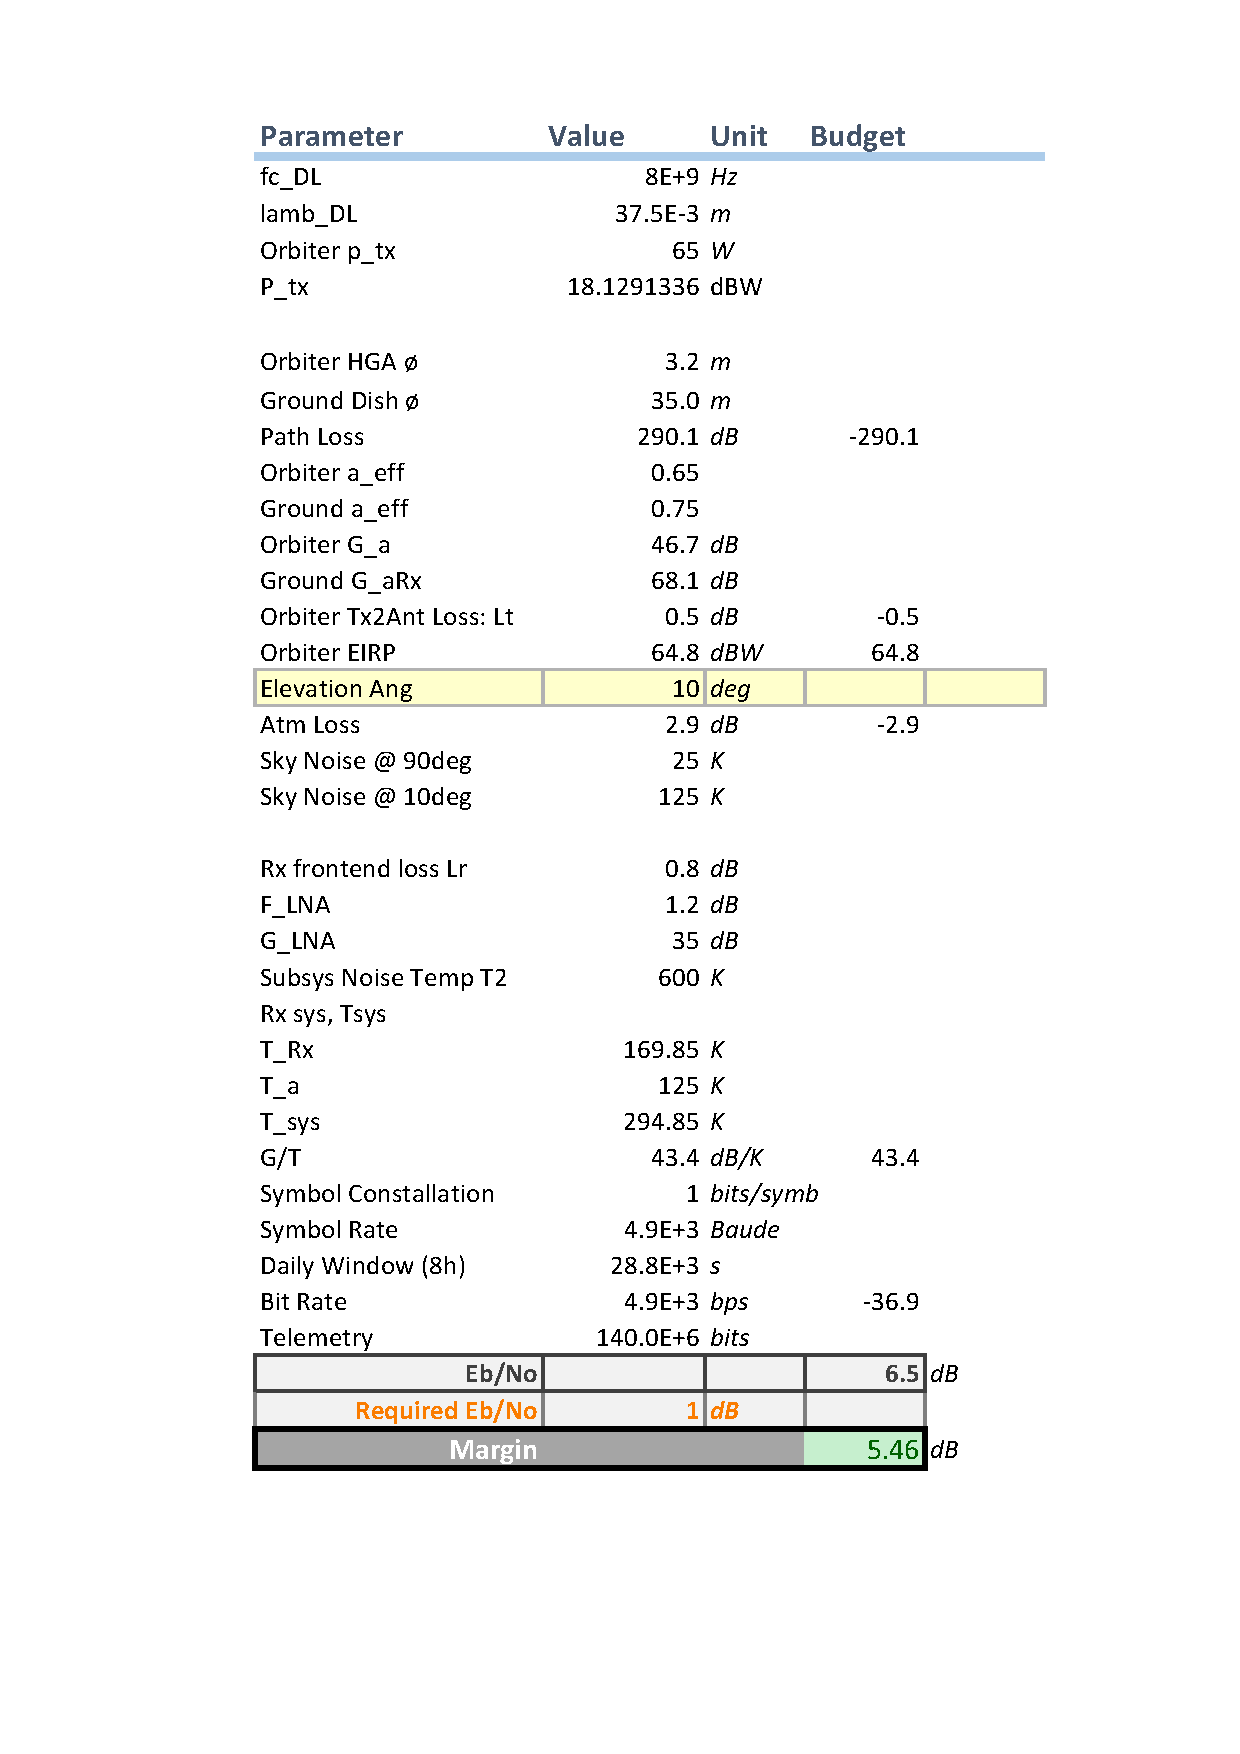
\includegraphics[width=.48\textwidth]{figures/comms/linkBudget-Xband}
		\label{fig:budget-X}
	}
	\subfloat[Ka-band link budget]{
		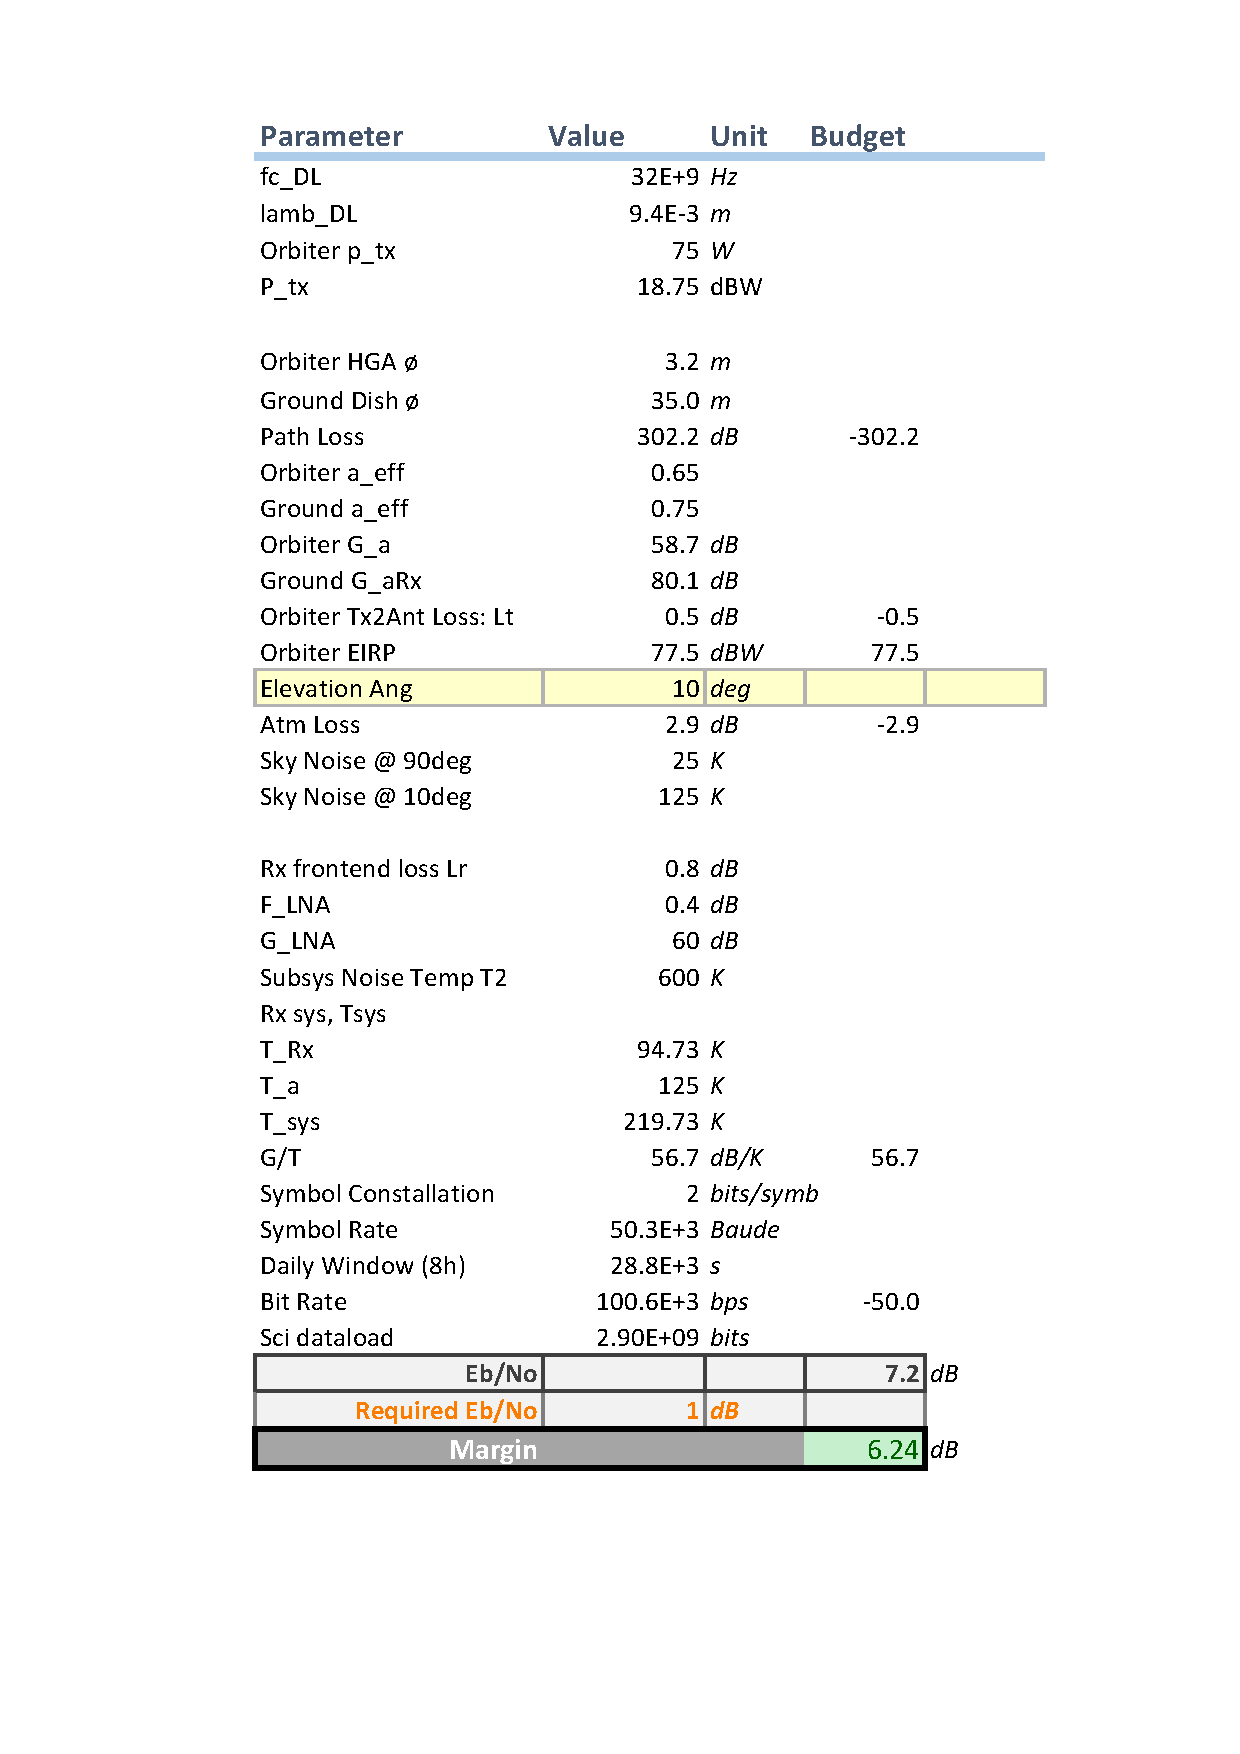
\includegraphics[width=.48\textwidth]{figures/comms/linkBudget-Kband}
		\label{fig:budget-K}
	}
	\caption{Link budget for X- and Ka-band}
\end{figure}
